\documentclass{article}\usepackage[]{graphicx}\usepackage[]{xcolor}
% maxwidth is the original width if it is less than linewidth
% otherwise use linewidth (to make sure the graphics do not exceed the margin)
\makeatletter
\def\maxwidth{ %
  \ifdim\Gin@nat@width>\linewidth
    \linewidth
  \else
    \Gin@nat@width
  \fi
}
\makeatother

\definecolor{fgcolor}{rgb}{0.345, 0.345, 0.345}
\newcommand{\hlnum}[1]{\textcolor[rgb]{0.686,0.059,0.569}{#1}}%
\newcommand{\hlstr}[1]{\textcolor[rgb]{0.192,0.494,0.8}{#1}}%
\newcommand{\hlcom}[1]{\textcolor[rgb]{0.678,0.584,0.686}{\textit{#1}}}%
\newcommand{\hlopt}[1]{\textcolor[rgb]{0,0,0}{#1}}%
\newcommand{\hlstd}[1]{\textcolor[rgb]{0.345,0.345,0.345}{#1}}%
\newcommand{\hlkwa}[1]{\textcolor[rgb]{0.161,0.373,0.58}{\textbf{#1}}}%
\newcommand{\hlkwb}[1]{\textcolor[rgb]{0.69,0.353,0.396}{#1}}%
\newcommand{\hlkwc}[1]{\textcolor[rgb]{0.333,0.667,0.333}{#1}}%
\newcommand{\hlkwd}[1]{\textcolor[rgb]{0.737,0.353,0.396}{\textbf{#1}}}%
\let\hlipl\hlkwb

\usepackage{framed}
\makeatletter
\newenvironment{kframe}{%
 \def\at@end@of@kframe{}%
 \ifinner\ifhmode%
  \def\at@end@of@kframe{\end{minipage}}%
  \begin{minipage}{\columnwidth}%
 \fi\fi%
 \def\FrameCommand##1{\hskip\@totalleftmargin \hskip-\fboxsep
 \colorbox{shadecolor}{##1}\hskip-\fboxsep
     % There is no \\@totalrightmargin, so:
     \hskip-\linewidth \hskip-\@totalleftmargin \hskip\columnwidth}%
 \MakeFramed {\advance\hsize-\width
   \@totalleftmargin\z@ \linewidth\hsize
   \@setminipage}}%
 {\par\unskip\endMakeFramed%
 \at@end@of@kframe}
\makeatother

\definecolor{shadecolor}{rgb}{.97, .97, .97}
\definecolor{messagecolor}{rgb}{0, 0, 0}
\definecolor{warningcolor}{rgb}{1, 0, 1}
\definecolor{errorcolor}{rgb}{1, 0, 0}
\newenvironment{knitrout}{}{} % an empty environment to be redefined in TeX

\usepackage{alltt}
\usepackage[a4paper, total={6.5in, 10.5in}]{geometry}

\author{Katarzyna Macioszek, Ada Majchrzak}
\title{Data Mining project - part I}
\IfFileExists{upquote.sty}{\usepackage{upquote}}{}
\begin{document}
\maketitle

\section{Introduction}

In this project, we will use data mining methods to perform analysis of \textit{Spambase}
dataset. The considered dataset was created from two collections of e-mails, 
the first being a set of non-spam personal and professional e-mails, and the 
second one coming from individuals who had filed spam. The e-mails were 
analyzed in terms of frequency of appearance of 54 selected words, numbers and characters,
and also in terms of the number of capital letters present. 
Those statistics were then collected into table and each record was labeled 
as spam or non-spam. Our goal is to first extract interesting and insightful data characteristics
by Exploratory Data Analysis procedures (plots, summary statistics), and then to perform a classification task,
distinguishing spam from non-spam. For the second part, we will compare the performance
of several methods, namely Linear Discriminant Analysis (LDA), Quadratic Discriminant Analysis (QDA),
K-Nearest Neighbours (KNN), and Random Forest. We will also evaluate those methods on different sets of features.
The benefit from this kind of study could be obtaining a model effective in terms 
of spam filtering. We know that spam e-mails are a very common problem in modern 
world, and although every mailbox nowadays has built-in filter for that kind
of content, non of them are completely accurate, so it is certainly a good idea
to keep studying this topic.

\section{Exploratory Data Analysis}



The dataset consist of 4601 records, none of which contain any missing values.
There are 57 numerical features and one categorical, \textit{type}, being a target class.
The target class takes two values -- spam and nonspam. As we can see from Figure \ref{fig1},
the classes are quite well balanced. Around 60\% of the records fall into nonspam category,
and about 40\% of them are spam. As for the numerical features, they can be divided into two
groups -- 54 features containing information about the frequency of selected words, numbers and 
special characters, expressed as percentage (further called Frequency features), 
and 3 features containing information about the capital letters in the e-mail (further called Capital features):

\begin{itemize}
  \item capitalAve -- average length of an uninterrupted sequence of capital letters,
  \item capitalLong -- length of longest uninterrupted sequence of capital letters,
  \item capitalTotal -- total number of capital letters.
\end{itemize}
Basic summary statistics for the numerical features can be found in Table \ref{tab1}.
The maximum frequency found in the dataset equals 42.8, and it is observed for \textit{num3d} variable. 
In general, the values for Frequency features are really low -- in most of the cases, even the $3^{rd}$
quartile is very close to 0, or even equal to 0, which suggest that the identification of 
potential outliers might prove challenging. There are only two variables of that type
for which the $3^{rd}$ quartile exceeds 1 -- \textit{you} (2.6) and \textit{your} (1.3).
Of course, this data stucture results in quite small standard deviations for the Frequency features.
Regarding Capital features, here the range of values is significantly broader. The minimum for all
three of those is 1, while the maximum is 1102.5 for \textit{capitalAve}, 9989.0 for \textit{capitalLong},
and 15841.0 for \textit{capitalTotal}. As expected, also the standard deviations for this set
of features are much higher compared to the previous one. Those differences need to be
kept in mind and accounted for during the classfication tasks.



\begin{knitrout}
\definecolor{shadecolor}{rgb}{0.969, 0.969, 0.969}\color{fgcolor}\begin{figure}[h]
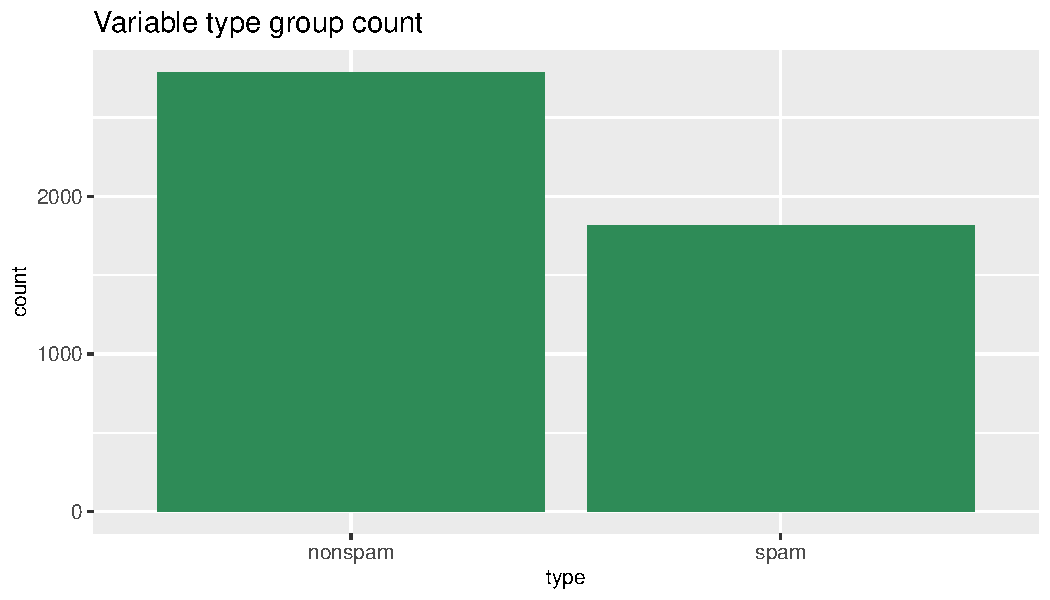
\includegraphics[width=\maxwidth]{figure/tgtClassPlot-1} \caption[\label{fig1} Target class distribution]{\label{fig1} Target class distribution}\label{fig:tgtClassPlot}
\end{figure}

\end{knitrout}


% latex table generated in R 4.3.1 by xtable 1.8-4 package
% Fri Nov 17 20:05:25 2023
\begin{table}[ht]
\centering
\begin{tabular}{rrrrrrrr}
  \hline
 & Mean & Std.Dev & Min & Max & Q1 & Median & Q3 \\ 
  \hline
address & 0.21 & 1.29 & 0.00 & 14.28 & 0.00 & 0.00 & 0.00 \\ 
  addresses & 0.05 & 0.26 & 0.00 & 4.41 & 0.00 & 0.00 & 0.00 \\ 
  all & 0.28 & 0.50 & 0.00 & 5.10 & 0.00 & 0.00 & 0.42 \\ 
  business & 0.14 & 0.44 & 0.00 & 7.14 & 0.00 & 0.00 & 0.00 \\ 
  capitalAve & 5.19 & 31.73 & 1.00 & 1102.50 & 1.59 & 2.28 & 3.71 \\ 
  capitalLong & 52.17 & 194.89 & 1.00 & 9989.00 & 6.00 & 15.00 & 43.00 \\ 
  capitalTotal & 283.29 & 606.35 & 1.00 & 15841.00 & 35.00 & 95.00 & 266.00 \\ 
  charDollar & 0.08 & 0.25 & 0.00 & 6.00 & 0.00 & 0.00 & 0.05 \\ 
  charExclamation & 0.27 & 0.82 & 0.00 & 32.48 & 0.00 & 0.00 & 0.32 \\ 
  charHash & 0.04 & 0.43 & 0.00 & 19.83 & 0.00 & 0.00 & 0.00 \\ 
  charRoundbracket & 0.14 & 0.27 & 0.00 & 9.75 & 0.00 & 0.06 & 0.19 \\ 
  charSemicolon & 0.04 & 0.24 & 0.00 & 4.38 & 0.00 & 0.00 & 0.00 \\ 
  charSquarebracket & 0.02 & 0.11 & 0.00 & 4.08 & 0.00 & 0.00 & 0.00 \\ 
  conference & 0.03 & 0.29 & 0.00 & 10.00 & 0.00 & 0.00 & 0.00 \\ 
  credit & 0.09 & 0.51 & 0.00 & 18.18 & 0.00 & 0.00 & 0.00 \\ 
  cs & 0.04 & 0.36 & 0.00 & 7.14 & 0.00 & 0.00 & 0.00 \\ 
  data & 0.10 & 0.56 & 0.00 & 18.18 & 0.00 & 0.00 & 0.00 \\ 
  direct & 0.06 & 0.35 & 0.00 & 4.76 & 0.00 & 0.00 & 0.00 \\ 
  edu & 0.18 & 0.91 & 0.00 & 22.05 & 0.00 & 0.00 & 0.00 \\ 
  email & 0.18 & 0.53 & 0.00 & 9.09 & 0.00 & 0.00 & 0.00 \\ 
  font & 0.12 & 1.03 & 0.00 & 17.10 & 0.00 & 0.00 & 0.00 \\ 
  free & 0.25 & 0.83 & 0.00 & 20.00 & 0.00 & 0.00 & 0.10 \\ 
  george & 0.77 & 3.37 & 0.00 & 33.33 & 0.00 & 0.00 & 0.00 \\ 
  hp & 0.55 & 1.67 & 0.00 & 20.83 & 0.00 & 0.00 & 0.00 \\ 
  hpl & 0.27 & 0.89 & 0.00 & 16.66 & 0.00 & 0.00 & 0.00 \\ 
  internet & 0.11 & 0.40 & 0.00 & 11.11 & 0.00 & 0.00 & 0.00 \\ 
  lab & 0.10 & 0.59 & 0.00 & 14.28 & 0.00 & 0.00 & 0.00 \\ 
  labs & 0.10 & 0.46 & 0.00 & 5.88 & 0.00 & 0.00 & 0.00 \\ 
  mail & 0.24 & 0.64 & 0.00 & 18.18 & 0.00 & 0.00 & 0.16 \\ 
  make & 0.10 & 0.31 & 0.00 & 4.54 & 0.00 & 0.00 & 0.00 \\ 
  meeting & 0.13 & 0.77 & 0.00 & 14.28 & 0.00 & 0.00 & 0.00 \\ 
  money & 0.09 & 0.44 & 0.00 & 12.50 & 0.00 & 0.00 & 0.00 \\ 
  num000 & 0.10 & 0.35 & 0.00 & 5.45 & 0.00 & 0.00 & 0.00 \\ 
  num1999 & 0.14 & 0.42 & 0.00 & 6.89 & 0.00 & 0.00 & 0.00 \\ 
  num3d & 0.07 & 1.40 & 0.00 & 42.81 & 0.00 & 0.00 & 0.00 \\ 
  num415 & 0.05 & 0.33 & 0.00 & 4.76 & 0.00 & 0.00 & 0.00 \\ 
  num650 & 0.12 & 0.54 & 0.00 & 9.09 & 0.00 & 0.00 & 0.00 \\ 
  num85 & 0.11 & 0.53 & 0.00 & 20.00 & 0.00 & 0.00 & 0.00 \\ 
  num857 & 0.05 & 0.33 & 0.00 & 4.76 & 0.00 & 0.00 & 0.00 \\ 
  order & 0.09 & 0.28 & 0.00 & 5.26 & 0.00 & 0.00 & 0.00 \\ 
  original & 0.05 & 0.22 & 0.00 & 3.57 & 0.00 & 0.00 & 0.00 \\ 
  our & 0.31 & 0.67 & 0.00 & 10.00 & 0.00 & 0.00 & 0.38 \\ 
  over & 0.10 & 0.27 & 0.00 & 5.88 & 0.00 & 0.00 & 0.00 \\ 
  parts & 0.01 & 0.22 & 0.00 & 8.33 & 0.00 & 0.00 & 0.00 \\ 
  people & 0.09 & 0.30 & 0.00 & 5.55 & 0.00 & 0.00 & 0.00 \\ 
  pm & 0.08 & 0.43 & 0.00 & 11.11 & 0.00 & 0.00 & 0.00 \\ 
  project & 0.08 & 0.62 & 0.00 & 20.00 & 0.00 & 0.00 & 0.00 \\ 
  re & 0.30 & 1.01 & 0.00 & 21.42 & 0.00 & 0.00 & 0.11 \\ 
  receive & 0.06 & 0.20 & 0.00 & 2.61 & 0.00 & 0.00 & 0.00 \\ 
  remove & 0.11 & 0.39 & 0.00 & 7.27 & 0.00 & 0.00 & 0.00 \\ 
  report & 0.06 & 0.34 & 0.00 & 10.00 & 0.00 & 0.00 & 0.00 \\ 
  table & 0.01 & 0.08 & 0.00 & 2.17 & 0.00 & 0.00 & 0.00 \\ 
  technology & 0.10 & 0.40 & 0.00 & 7.69 & 0.00 & 0.00 & 0.00 \\ 
  telnet & 0.06 & 0.40 & 0.00 & 12.50 & 0.00 & 0.00 & 0.00 \\ 
  will & 0.54 & 0.86 & 0.00 & 9.67 & 0.00 & 0.10 & 0.80 \\ 
  you & 1.66 & 1.78 & 0.00 & 18.75 & 0.00 & 1.31 & 2.64 \\ 
  your & 0.81 & 1.20 & 0.00 & 11.11 & 0.00 & 0.22 & 1.27 \\ 
   \hline
\end{tabular}
\caption{Summary statistics for numerical features} 
\label{tab1}
\end{table}



\end{document}
